\documentclass[a4paper]{article}

    %% Language and font encodings
    \usepackage[english]{babel}
    \usepackage[utf8x]{inputenc}
    \usepackage[T1]{fontenc}
    \usepackage{listings}
    \usepackage{color}
    \usepackage{hyperref}
    \usepackage{multicol}
    \usepackage{mwe}
    
    \definecolor{dkgreen}{rgb}{0,0.6,0}
    \definecolor{gray}{rgb}{0.5,0.5,0.5}
    \definecolor{mauve}{rgb}{0.58,0,0.82}
    
    \lstset{frame=tb,
      language=Java,
      aboveskip=3mm,
      belowskip=3mm,
      showstringspaces=false,
      columns=flexible,
      basicstyle={\small\ttfamily},
      numbers=none,
      numberstyle=\tiny\color{gray},
      keywordstyle=\color{blue},
      commentstyle=\color{dkgreen},
      stringstyle=\color{mauve},
      breaklines=true,
      breakatwhitespace=true,
      tabsize=3
    }
    
    %% Sets page size and margins
    \usepackage[a4paper,top=3cm,bottom=2cm,left=3cm,right=3cm,marginparwidth=1.75cm]{geometry}
    
    %% Useful packages
    \usepackage{amsmath}
    \usepackage{graphicx}
    \usepackage[colorinlistoftodos]{todonotes}
    % \usepackage[colorlinks=true, allcolors=blue]{hyperref}
    
    \title{Wave: A PIC/FLIP Fluid Simulator}
    \author{Jonathan Lee}
    \date{}
    
    \begin{document}
    \maketitle
    
    \begin{figure*}[ht!]
    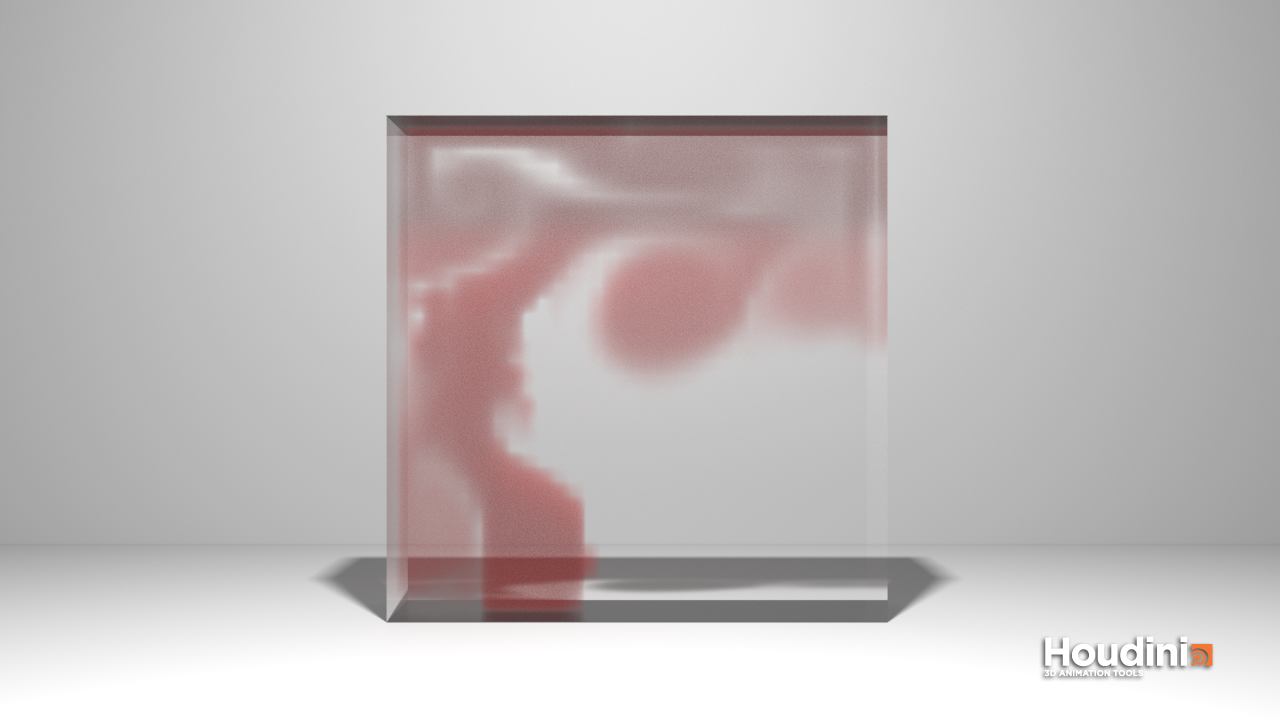
\includegraphics[width=.3\textwidth]{_smoke.png}\hfill
    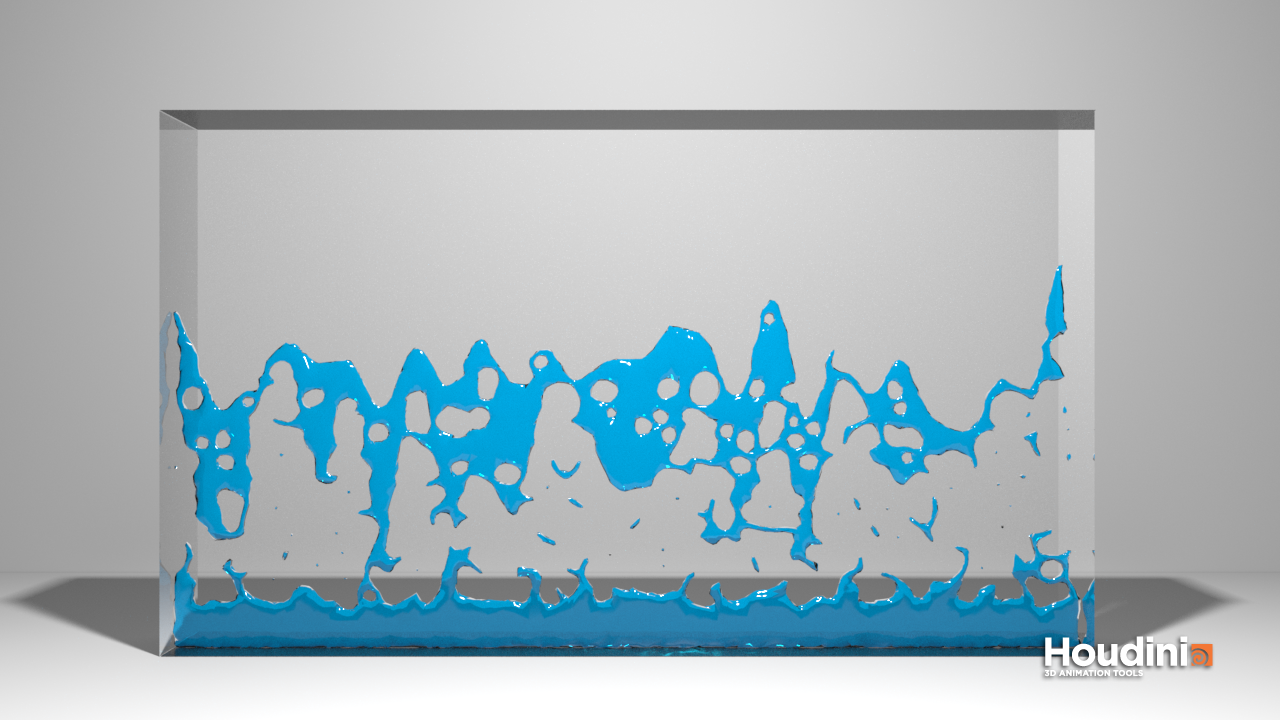
\includegraphics[width=.3\textwidth]{_2d.png}\hfill
    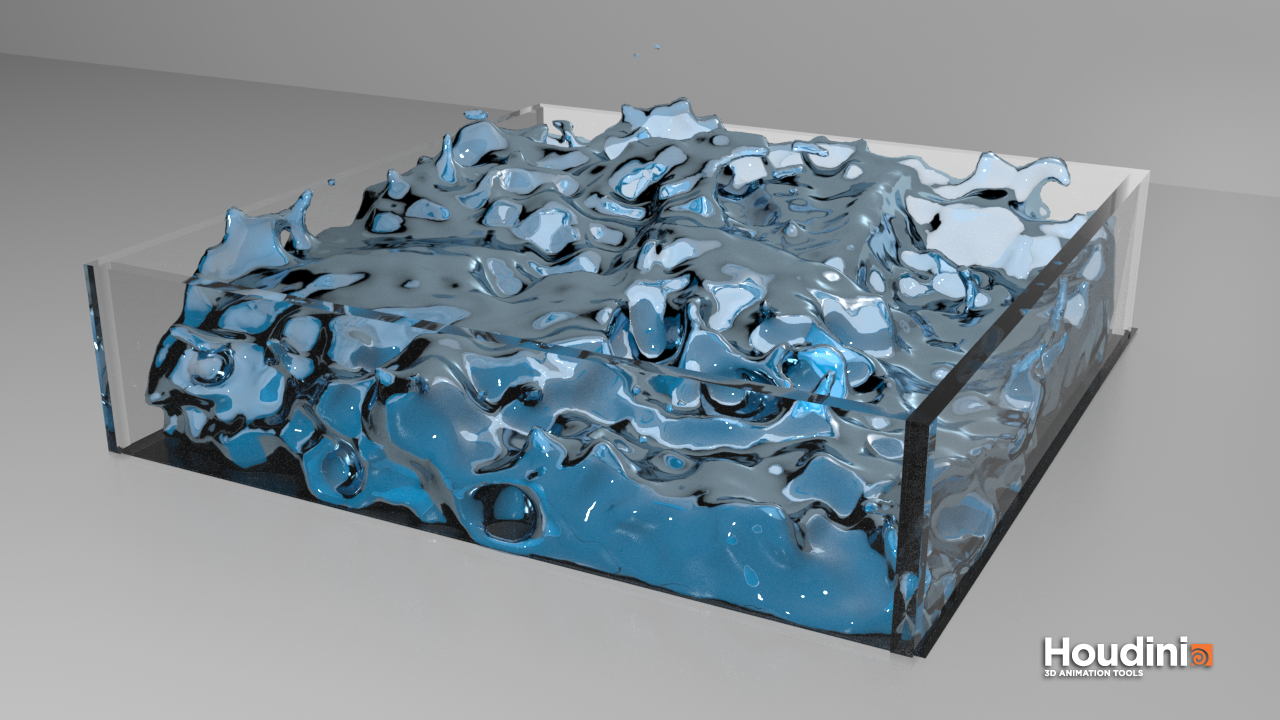
\includegraphics[width=.3\textwidth]{_3d.png}
    \end{figure*}
    
    \section{Introduction}
    Wave is a hybrid simulator that soles equations using Lagrangian and Eulerian views. There are two simulation modes: Smoke and Fluid. The smoke simulator is an Eulerian solver where all the calculations are performed on the grid whereas the fluid simulator combines the Eulerian calculations with the Lagrangian calculations on particles. 
    
    \begin{itemize}
    \item{\href{https://youtu.be/yL-t_XStaGg}{Smoke Demo 1}}
    \item{\href{https://youtu.be/JgeTdxtrdic}{Smoke Demo 2}}
    \item{\href{https://youtu.be/dJZmWV0ZABQ}{Fluid Demo 1}}
    \item{\href{https://youtu.be/V1Y69BMAeaE}{Fluid Demo 2}}
    \end{itemize}
    
    \section{Smoke}
    Wave's smoke simulator is based on Bridson's 2007 Siggraph course notes. 
    
    \subsection{Algorithm}
    \begin{lstlisting}
    For each time step:
        Update sources
        
        // Calculate new velocities
        Advect velocity
        Add external forces
        Project pressure
        
        // Calculate temperature
        Advect temperature
    \end{lstlisting}
    
    \subsubsection{Velocity Advection}
    The goal here is to find the new velocities on the grid. A semi-Lagrangian approach was used to to solve the material derivative $ Dq / Dt $. To do this, we loop over the faces to find the implicit particle's starting position. Once found, we can interpolate on the grid to find the new velocity. 
    
    \subsubsection{External Forces}
    For a smoke simulation, we only account for two external forces: buoyancy and vorticity. 
    
    \subsubsection*{Buoyancy}
    The buoyancy force is what allows the smoke to rise when the temperature is hot and fall when the temperature is low. Instead of calculating the gravitational force, we substitute that for the buoyancy force. Each face on the Y velocity grid gets updated with this force. 
    \[ f_{buoy} = (0, \alpha s - \beta(T - T_{amb}), 0) \]
    
    \subsubsection*{Vorticity Confinement}
    Vorticity confinement allows the smoke to be more lively and energetic as it prevents the vortices from disappearing too quickly.
    
    \noindent New grids are created to keep track of the vorticity of each direction as well as one to hold the vorticity magnitudes at the cells.
    
    \noindent Vorticity is defined as
    \[ \vec{\omega}^{\,} = \nabla \times \vec{u}^{\,} \] \newline
    \noindent but is discretized as 
    \[ \vec{\omega}^{\,}_{i, j, k} = (\frac{w_{i,j+1,k} - w_{i,j-1,k}}{2\Delta x} - \frac{v_{i,j,k+1} - v_{i,j,k-1}}{2\Delta x},\]
    \[\frac{u_{i,j,k+1} - u_{i,j,k-1}}{2\Delta x} - \frac{w_{i+1,j,k} - v_{i-1,j,k}}{2\Delta x}\]
    \[\frac{v_{i+1,j,k} - v_{i-1,j,k}}{2\Delta x} - \frac{u_{i,j+1,k} - u_{i,j-1,k}}{2\Delta x}) \]
    
    \noindent The vorticity gradient gets computed using central differences
    \[ \vec{N}^{\,}_{i,j,k} = \frac{\nabla |{\vec{\omega}^{\,}}|_{i,j,k}}{|{|{\nabla |{\vec{\omega}^{\,}}|_{i,j,k}}|}| + 10^{{-20}}} \]
    
    \noindent Vorticity confinement is defined as
    \[ f_{conf} = \epsilon \Delta x(\vec{N}^{\,} \times \vec{w}^{\,}) \]
    
    \noindent To apply the confinement force, we take the average of both faces of the cell. For example if we're on the $ mU $ grid, we add $ f_{conf}.x $ to $ mU $ and divide it by $ 2 $ to account for $ i $ and $ i + 1 $.
    
    \subsubsection{Pressure Projection}
    Projection allows for the simulation to be divergence free and solves for incompressibility. It solves the equation $ Ap = d $.
    
    \begin{lstlisting}
    Calculate divergence d
    Calculate A matrix
    Create MIC preconditioner
    Solve Ap = d with PCG
    Compute new velocities using the pressure gradient
    \end{lstlisting}
    
    \subsubsection*{Divergence}
    Divergence determines how much fluid is going in and out of the cell. 
    \[ d(i, j, k) = -\frac{u_{i+1/2,j,k} - u_{i - 1/2,j,k}}{\Delta x} + \frac{v_{i,j+1/2,k} - v_{i,j-1/2,k}}{\Delta x} + \frac{w_{i,j,k+1/2} - w_{i,j,k-1/2}}{\Delta x} \]
    
    \noindent If the cell face lies on the border of the MAC grid, that component's contribution is 0.
    
    \subsubsection*{Preconditioner}
    The Modified Incomplete Cholesky Preconditioner is based on the algorithm presented in the course notes on page 36. It calculates the value for each fluid cell.
    
    \subsection*{Pressure Update}
    The preconditioner fills the initial pressures into the grid. To really solve for pressure, we have to divide by the pressure constant $ \frac{\Delta t}{\rho * dx * dx} $ because of the way the A matrix is set up.
    
    \subsubsection*{Computing new velocities}
    To compute the new velocities, we loop through each of the faces on the grid $u, v, w$. Faces that are on boundaries get set to 0, otherwise their velocity values get updated as follows:
    
    \[ u^{n+1}_{i+1/2,j,k} = u_{i+1/2,j,k} - \Delta t \frac{1}{\rho} \frac{p_{i+1,j,k} - p_{i,j,k}}{\Delta x}\]
    \[ v^{n+1}_{i,j+1/2,k} = v_{i,j+1/2,k} - \Delta t \frac{1}{\rho} \frac{p_{i,j+1,k} - p_{i,j,k}}{\Delta x}\]
    \[ w^{n+1}_{i,j,k+1/2} = w_{i,j,k+1/2} - \Delta t \frac{1}{\rho} \frac{p_{i,j,k+1} - p_{i,j,k}}{\Delta x}\]
    
    \subsection{Temperature Advection}
    Temperature advection is similar to advecting velocities. Since temperature is contained at the centers of the grid, we can loop through the cells to get the new value. We can get the center of the grid cell, then integrate it using RK2 or RK4, and finally use the start position to get the new temperature.
    
    \section{Fluids}
    \textbf{PIC} is a simulation method where we calculate everything except advection on the grid and advection on particle s (Lagrangian). There are two main steps in PIC: particle velocity to grid transfer and grid velocity to particle transfer. \newline
    \noindent \textbf{FLIP} is a simulation method where everything is solved on the grid (Eulerian). Rather than advecting particles based on previous positions, FLIP updates velocities on the grid by taking the difference between grids. 
    
    \subsection{Algorithm}
    Wave's fluid simulator is mainly based on Zhu and Bridson's 2005 PIC/FLIP algorithm presented in "Animating Sand as a Fluid" with some other references listed below. 
    \begin{lstlisting}
    Initialize particles
    For each time step:
        Update marker grid
        
        Particle to grid transfer	// PIC
        FLIP velocity save			// FLIP
    
        // Non advection steps
        Add external forces
        Set boundary conditions
        Project pressure
        
        // Update velocities
        Update FLIP velocity save	// FLIP
        Grid to particle transfer	// PIC
        
        //Move particle
        Advect particle
    \end{lstlisting}
    
    \subsection{Data Storage}
    \subsubsection{Marker Grid}
    One of the most important aspects of creating a fluid simulation is the marker grid. Each cell that has a face along the boundaries is marked as a SOLID. If there is a particle in a cell, said cell gets marked as a FLUID. All other cells are marked as AIR. The marker grid gets updated each step during the simulation.
    
    \subsubsection{Velocity Grids}
    We need to store two different velocity grids in order to do FLIP and PIC updates. \newline
    \begin{itemize}
      \item Main Grid: \textbf{\textit{mU}}, \textbf{\textit{mV}}, \textbf{\textit{mW}}
      \item FLIP Grid: \textbf{\textit{mUcopy}}, \textbf{\textit{mVcopy}}, \textbf{\textit{mWcopy}}
    \end{itemize}
    
    \subsubsection{Particles}
    Like the velocity grids, we need several vectors for particles, one for PIC, FLIP, and PIC/FLIP.
    \begin{itemize}
        \item particlesFLIP: Gets updated in updateVelFLIP
        \item particlesPIC: Gets updated in gridToParticle 
        \item particles: Gets updated in advectParticle
    \end{itemize}
    
    \subsection{Particles}
    A particle class was created and contains position and velocity. When initialized, the user must define its container size. This container size is different from theDim in that it dictates how large the fluid will start and where the particles will spawn. The positions are randomized within a grid cell and the velocity starts at 0. 
    
    \subsection{Particle Velocity to Grid Transfer}
    Essentially, we have to get a weighted average of nearby particle velocities. Bridson proposed the following algorithm:
    \begin{lstlisting}
    Loop over particle index p:
    // x_p is the particle index
    // x_ijk is the grid cell with respect to the velocity face
    // W is the sum of the kernels
        Loop over grid indices i, j, k where kernel(x_p - x_ijk) is non-zero
            Add velocity * kernel(x_p - x_ijk) / W
    \end{lstlisting}
    
    \[ x = particlePos.x - (index.x * cellSize)\]
    \[ kernel(x, y, z) = h(\frac{x}{\Delta x}) h(\frac{y}{\Delta y}) h(\frac{z}{\Delta z}) \]
    \[ kernelHelper(r) = (abs(r) <= 1) ? 1 - abs(r) \]
    
    \noindent Rather than doing a loop over all grid cells where there is a non-zero kernel, I just used neighboring grid cells.
    
    \noindent Once the values are calculated, the velocity faces get updated.
    
    \subsection{FLIP Save}
    After averaging particle velocities with respect to neighboring faces, we save the face velocities into the \textbf{\textit{copy}} grids.
    
    \subsection{External Forces}
    The only external force taken into account for this is gravity. This is simply adding a gravitational force to the $y-$component of $mV$.
    
    \subsection{Boundary Conditions}
    The faces that surround a SOLID cell have their velocities reset to 0. For example:
    \begin{lstlisting}
    FOR EACH CELL
        if(i == 0) // inherent since the marker grid labels 0 and theDim[X] as SOLID
            mU(0, j, k) = 0;
            mU(1, j, k) = 0;
    \end{lstlisting}
    
    \subsection{Pressure Projection}
    I ran into issues with the provided A matrix and PCG solvers. It should have been a simple modification. The A matrix is filled for each fluid cell, the pressure matrix gets filled at fluid cells, and velocity gets updated based on the cell and the neighboring cell. Because I don't understand in much detail how PCG or MIC works, I used Eigen for this specific case. 
    
    \subsection{FLIP Velocity Update}
    The previously saved velocity grids get updated by subtracting the grids updated after the non-advection steps. This is done by subtracting the updated grid from the FLIP copy grid. Using this newly calculated grid, we can update the particles for FLIP (important for lerping between PIC and FLIP). 
    \begin{lstlisting}
    FOR EACH FACE
        mUcopy(i, j, k) = mU(i, j, k) - mUcopy(i, j, k)
        update particlesFLIP with mUcopy
    \end{lstlisting}
    
    \subsection{Grid to Particle Transfer}
    A PIC particles container gets updated based on the main velocity grids. Because all the calculate is done on the main grid, we can simply integrate to get the new particle velocities. 
    
    \subsection{Particle Advection}
    Here is where we lerp between PIC and FLIP. With this new updated velocity, we can get the new particle position using RK2 or RK4.
    \[ flipPercentage = .95 \]
    \[ particleVel = ((1 - flipPercentage) * particleVelPIC) + (flipPercentage * particleVelFLIP \] 
    
    \bibliography{sample}
    \begin{thebibliography}{9}
    
    \bibitem{latexcompanion} 
    Robert Bridson and Matthias Muller-Fischer.
    \textit{Fluid Simulation Course Notes}. Siggraph, 2007.
    
    \bibitem{latexcompanion} 
    Yongning Zhu and Robert Bridson.
    \textit{Animating Sand as Fluid}. 2005.
    
    \bibitem{latexcompanion} 
    David Cline David Cardon Parris K. Egbert.
    \textit{Fluid Flow for the Rest of Us: Tutorial of the Marker and Cell Method in
    Computer Graphics}. 2005.
    
    \bibitem{latexcompanion} 
    Ioannis Ioannidis.
    \textit{3D Particle in Cell / Fluid Implicit Particle Fluid Solver using OpenMP directives}. 2012.
    \end{thebibliography}
    \end{document}